\chapter{Thermostat System Function}
\label{chap:thermostat-system-function}

The Thermostat performs two logically independent functions. The first regulates the Current
Temperature in the Isolette so it is maintained within the Desired Temperature Range. The
second monitors the Current Temperature in the Isolette and activates an Alarm if it falls below
or rises above the Alarm Temperature Range.

The high-level requirements for the Thermostat Function are as follows:

\begin{itemize}
\item REQ-TH-1: The Thermostat shall set the value of the Heat Control.

      Rationale: A primary function of the Thermostat is to turn the Heat Control on and off to
      maintain the Current Temperature in the Isolette within the Desired Temperature Range,
      which is required by SR-1.
\item REQ-TH-2: The Thermostat Function shall set the value of the Regulator Status.

      Rationale: SR-1 requires the Thermostat to provide an independent regulator function.
      The status of this function is provided to the Operator Interface by the Thermostat. The
      Operator Interface will use the Regulator Status and the Monitor Status to report the
      overall status of the Thermostat, which is required by SR-1.
\item REQ-TH-3: The Thermostat shall set the value of the Display Temperature.

      Rationale: The Current Temperature is displayed on the Operator Interface to provide
      the operators with an additional means to confirm the Isolette is maintaining the
      temperature correctly. This value is provided by the Thermostat to the Operator Interface
      as the Display Temperature.
\item REQ-TH-4: The Thermostat shall set the value of the Alarm Control.

      Rationale: A primary Thermostat Function is to activate the Alarm if the Isolette is
      unable to maintain the Current Temperature within the Alarm Temperature Range, which
      is required by SR-2.
\item REQ-TH-5: The Thermostat shall set the value of the Monitor Status.

      Rationale: SR-2 requires the Thermostat to provide an independent monitor function.
      The status of this function must be provided to the Operator Interface, which will use it
      and the status of the regulator function to report the overall status of the thermostat.
\end{itemize}

The Thermostat Function is allocated into subfunctions as shown in figure ~\ref{fig:dependency}.

\begin{figure*}[ht]
  \centerline{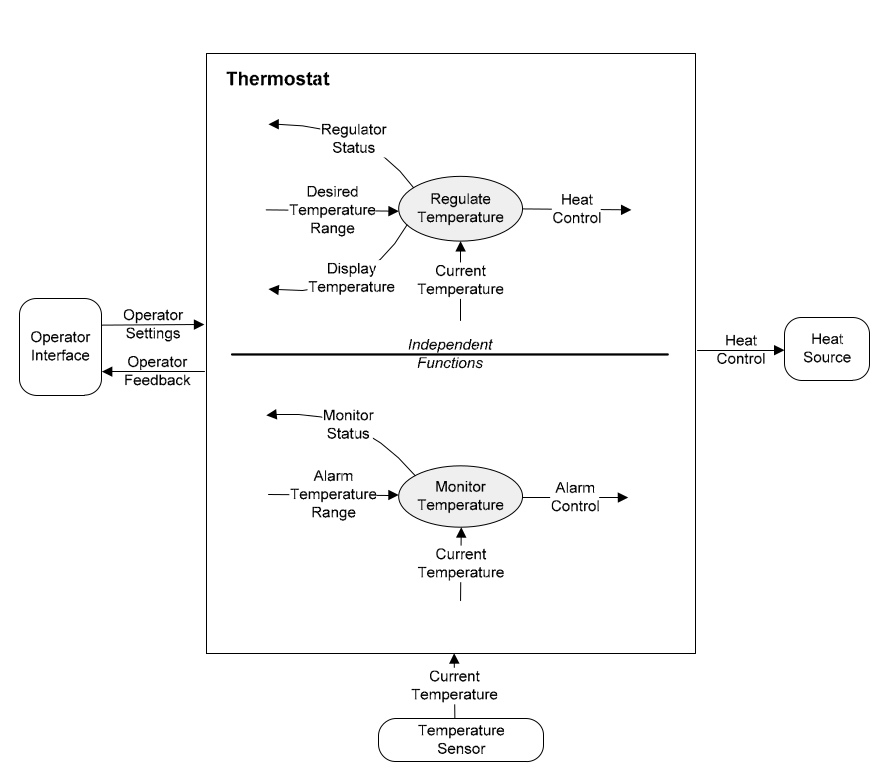
\includegraphics[width=\textwidth]{figures/thermostat-dependency-diagram.png}}
  \vspace{-.4cm}
  \caption{Thermostat Dependency Diagram}
  \vspace{-.4cm}
 \label{fig:dependency}
\end{figure*}

\section{Regulate Temperature Function}
\label{sec:regulate-temperature-function}

The Regulate Temperature Function compares the Current Temperature from the Temperature
Sensor with the Desired Temperature Range provided by the Operator Interface and turns the
Heat Source on or off to keep the Current Temperature within the Desired Temperature Range.
It also provides the Display Temperature and the Regulator Status back to the Operator Interface.

The high-level requirements for the Regulate Temperature Function are as follows:

\begin{itemize}
\item REQ-RT-1: The Regulate Temperature Function shall set the value of the Heat Control.

      Rationale: The primary function of the Regulate Temperature Function is to turn the
      Heat Control on and off to maintain the Current Temperature in the Isolette within the
      Desired Temperature Range, as required by SR-1.
\item REQ-RT-2: The Regulate Temperature Function shall set the value of the Regulator
      Status.

      Rationale: The status of the Regulate Temperature Function is provided to the Operator
      Interface so it can use the status of the Regulate Temperature and Monitor Temperature
      Functions to report the overall status of the Thermostat, as required by SR-1.
\item REQ-RT-3: The Regulate Temperature Function shall set the value of the Display
      Temperature.

      Rationale: The Current Temperature of the Isolette is displayed on the Operator Interface
      to provide the operators with an additional means to confirm that the Isolette is
      maintaining the temperature correctly. This value is provided by the Regulate
      Temperature Function to the Operator Interface as the Display Temperature.
\end{itemize}

The Regulate Temperature Function is allocated into subfunctions in figure ~\ref{fig:temp-dependency}.

\begin{figure*}[ht]
  \centerline{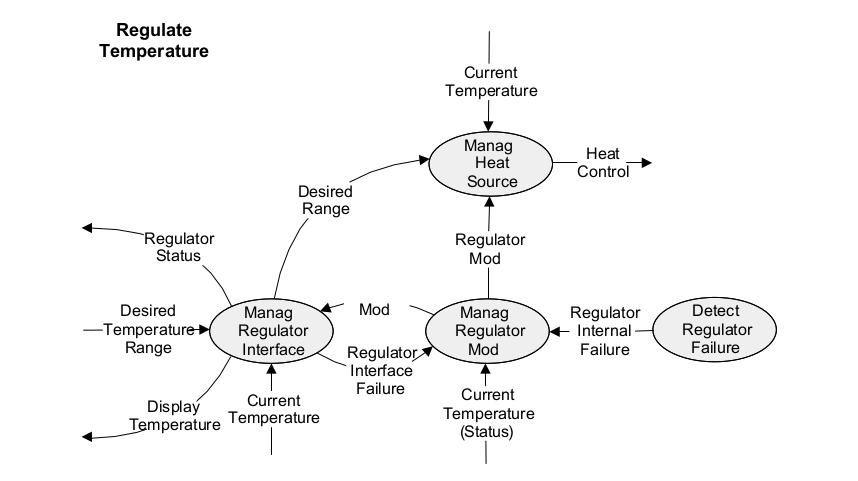
\includegraphics[width=\textwidth]{figures/regulate-temperature-dependency.png}}
  \vspace{-.4cm}
  \caption{Regulate Temperature Dependency Diagram}
  \vspace{-.4cm}
 \label{fig:temp-dependency}
\end{figure*}

The internal variables for the Regulate Temperature Function are shown in table ~\ref{tab:internal-variables}.

\begin{table}
\begin{tabular}{|l|l|l|l|l|}
\hline
Name & Type & Range & Units & Physical Interpretation \\\hline
Desired Temperature &  &  &  & Desired range of Isolette temperature \\\hline
Lower Desired Temperature & Integer & [96..101] & °F & Lower value of desired range \\\hline
Upper Desired Temperature & Integer & [97..102] & °F & Upper value of desired range \\\hline
Regulator Interface Failure & Boolean & False, True &  & Indicates an operator interface \\\hline
Regulator Internal Failure & Boolean & False, True &  & Indicates an internal failure \\\hline
Regulator Mode & Enumerated & Init &  & Initializing following power-up \\\cline{3-5}
  &  & NORMAL &  & Normal mode of operation \\\cline{3-5}
  &  & FAILED &  & Internal failure detected \\\hline
\end{tabular}
\caption{The Regulate Temperature Internal Variables}
\label{tab:internal-variables}
\end{table}

\subsection{Manage Regulator Interface Function}
\label{subsec:MRI-fun}

The Manage Regulator Interface Function defines the interaction with the Operator Interface
external entity. These include obtaining the Desired Range, reporting back the status of the
Regulate Temperature Function, and reporting back the Display Temperature. The constants are
shown in table ~\ref{tab:MRI-fun-constants}.

\begin{table}
\begin{tabular}{|l|l|l|l|l|}
\hline
Name & Type & Range & Units & Physical Interpretation \\\hline
Max Operator & Real & 0.5 & Sec & This time an operation will tolerate between an operator \\
Response Time &  &  &  & request or a change in the Thermostat state and the \\
  &  &  &  & visible response \\\hline
\multicolumn{5}{|l|}{Rationale: A trade study has shown that this lag should be no more than 0.5 second.} \\\hline
\end{tabular}
\caption{Manage Regulator Interface Function Constants}
\label{tab:MRI-fun-constants}
\end{table}

The requirements for the Regulator Status controlled variable are as follows:

\begin{itemize}
\item REQ-MRI-1: If the Regulator Mode is INIT, the Regulator Status shall be set to Init.
\item REQ-MRI-2: If the Regulator Mode is NORMAL, the Regulator Status shall be set to On.
\item REQ-MRI-3: If the Regulator Mode is FAILED, the Regulator Status shall be set to Failed.

      Latency: $<$ Max Operator Response Time
      Tolerance: N/A
\end{itemize}

The requirements for the Display Temperature controlled variable are as follows:

\begin{itemize}
\item REQ-MRI-4: If the Regulator Mode is NORMAL, the Display Temperature shall be set
      to the value of the Current Temperature rounded to the nearest integer.

      Rationale: Displaying the rounded value of the Current Temperature provides the the
      most accurate display of the Current Temperature possible using an integer display.
      When combined with the accuracy of the Temperature Sensor (EA-TS-2), the Display
      Temperature should be within 0.6°F of the actual value.
\item REQ-MRI-5: If the Regulator Mode is not NORMAL, the value of the Display Temperature is UNSPECIFIED.

      Rationale: In modes other than NORMAL, the value of Display Temperature is not
      meaningful and should not be used.

      Latency: $<$ Max Operator Response Time

      Tolerance: ±0.6°F
\end{itemize}

The requirements for the Regulator Interface Failure internal variable are as follows:

\begin{itemize}
\item REQ-MRI-6: If the Status attribute of the Lower Desired Temperature or the Upper
      Desired Temperature is Invalid, the Regulator Interface Failure shall be set to True.
\item REQ-MRI-7: If the Status attribute of the Lower Desired Temperature and the Upper
      Desired Temperature is Valid, the Regulator Interface Failure shall be set to False.

      Rationale: The Regulator Interface Failure internal variable indicates if any errors have
      occurred in sensing the Operator Interface monitored variables needed by the Regulate
      Temperature Function. Note that its initial value on power-up will always be True since
      the Status of the Lower Desired Temperature and the Upper Desired Temperature are
      initially Invalid.
\end{itemize}

The requirements for the Desired Range internal variable are as follows:

\begin{itemize}
\item REQ-MRI-8: If the Regulator Interface Failure is False, the Desired Range shall be set to
      the Desired Temperature Range.
\item REQ-MRI-9: If the Regulator Interface Failure is True, the Desired Range is UNSPECIFIED.

      Rationale: The Desired Range is only meaningful when there is not a Regulator Interface
      Failure. If there is, its value should not be used, and it can be set to any value.
\end{itemize}

\subsection{Manage Regulator Mode Function}
\label{subsec:MRM-fun}

The Manage Regulator Mode Function determines the mode of the Regulate Temperature
Function. The constants and definitions are shown in tables ~\ref{tab:MRM-fun-constants} and ~\ref{tab:MRM-fun-definitions}, respectively.

\begin{table}
\begin{tabular}{|l|l|l|l|l|}
\hline
Name & Type & Range & Units & Physical Interpretation \\\hline
Regulator & Real & 1.0 & Sec & The time allowed for initialization of the Regulate \\
Init Timeout &  &  &  & Temperature Function before declaring failure \\\hline
\multicolumn{5}{|l|}{Rationale: A trade study has shown that users become impatient if the Thermostat requires} \\
\multicolumn{5}{|l|}{more than one second to initialize.} \\\hline
\end{tabular}
\caption{The Manage Regulator Mode Function Constants}
\label{tab:MRM-fun-constants}
\end{table}

\begin{table}
\begin{tabular}{|l|l|l|}
\hline
Name & Type & Definition \\\hline
Regulator Status & Boolean & NOT (Regulator Interface Failure OR Regulator Internal Failure) \\
  &  & AND Current Temperature.Status = Valid \\\hline
\end{tabular}
\caption{The Manage Regulator Mode Function Definitions}
\label{tab:MRM-fun-definitions}
\end{table}

The requirements for the Regulator Mode internal variable are as follows:

\begin{itemize}
\item The modes and transitions of the Manage Regulator Mode Function are specified in the
      state transition diagram shown in figure ~\ref{fig:RTMT-diagram}. Each transition is a separate requirement
      and is assigned a unique identifier (e.g., Req MRM 1). All transitions are assumed to
      occur in negligible time.

      Rationale: (Req MRM 3 and Req MRM 4) Once the regulator has failed, the only way
      for it to re-enter normal operation is for it to be powered off and on. This ensures that the
      operators are made aware of any transient failures that the regulator may be experiencing.
\end{itemize}

\begin{figure*}[ht]
  \centerline{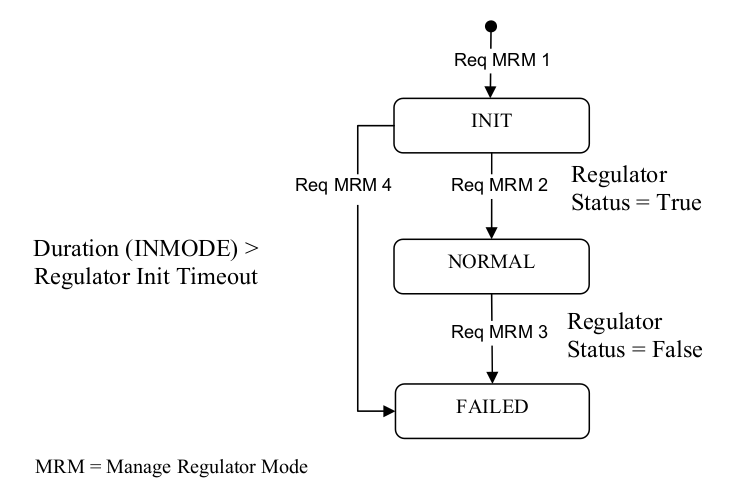
\includegraphics[width=\textwidth]{figures/regulate-temperature-mode-transition.png}}
  \vspace{-.4cm}
  \caption{Regulate Temperature Mode Transition Diagram}
  \vspace{-.4cm}
 \label{fig:RTMT-diagram}
\end{figure*}

\subsection{Manage Heat Source Function}
\label{subsec:manage-heat-source}

The Manage Heat Source Function turns the Heat Source on and off to maintain the Current
Temperature of the Isolette within the Desired Temperature Range. The constants are shown in
table ~\ref{tab:MHSF-constants}.

\begin{table}
\begin{tabular}{|l|l|l|l|l|}
\hline
Name & Type & Range & Units & Physical Interpretation \\\hline
Allowed Heat & Real & 6.0 & Sec & The maximum time by which the Heat Source \\
Source Latency &  &  &  & must be turned on or off to ensure acceptable  \\
  &  &  &  & Operation of the Isolette system \\\hline
\multicolumn{5}{|l|}{Since a closed Isolette will warm or cool at a maximum rate of 1°F per minute} \\
\multicolumn{5}{|l|}{(EA-IS1 and EA-IS2), turning the Heat Source on or off within 6 seconds ensures that the} \\
\multicolumn{5}{|l|}{Current Temperature will not have changed by more than 0.1°F, the required accuracy and} \\
\multicolumn{5}{|l|}{resolution of the Temperature Sensor (EA-TS2).} \\\hline
\end{tabular}
\caption{The Manage Heat Source Function Constants}
\label{tab:MHSF-constants}
\end{table}

The requirements for the Heat Control controlled variable are as follows:

\begin{itemize}
\item REQ-MHS-1: If the Regulator Mode is INIT, the Heat Control shall be set to Off.

      Rationale: A regulator that is initializing cannot regulate the Current Temperature of the
      Isolette and the Heat Control should be turned off.
\item REQ-MHS-2: If the Regulator Mode is NORMAL and the Current Temperature is less
      than the Lower Desired Temperature, the Heat Control shall be set to On.
\item REQ-MHS-3: If the Regulator Mode is NORMAL and the Current Temperature is
      greater than the Upper Desired Temperature, the Heat Control shall be set to Off.
\item REQ-MHS-4: If the Regulator Mode is NORMAL and the Current Temperature is
      greater than or equal to the Lower Desired Temperature and less than or equal to the
      Upper Desired Temperature, the value of the Heat Control shall not be changed.

      Rationale: When the Isolette is warming towards the Upper Desired Temperature, the
      Heat Source should be left on until the Upper Desired Temperature is reached. In a
      similar fashion, if the Isolette is cooling towards the Lower Desired Temperature, the
      Heat Source should be left off until the Lower Desired Temperature is reached.
\item REQ-MHS-5: If the Regulator Mode is FAILED, the Heat Control shall be set to Off.

      Rationale: In failed mode, the regulator cannot regulate the Current Temperature of the
      Isolette and the Heat Control should be turned off.

      Latency: $<$ Allowed Heat Source Latency

      Tolerance: N/A
\end{itemize}

\subsection{Detect Regulator Failure Function}
\label{subsec:detect-regulator-failure}

The Detect Regulator Failure Function identifies internal failures, (e.g., a memory check failure)
in the Regulate Temperature Function. It defines a single Boolean-valued internal variable,
Regulator Internal Failure, which is set to True if an internal failure is detected.

The requirements for Regulator Internal Failure variable are implementation-specific and cannot
be specified until an implementation platform is chosen.

\section{Monitor Temperature Function}
\label{sec:monitor-temperature}

The Monitor Temperature Function compares the Current Temperature from the Temperature
Sensor with the Alarm Temperature Range provided by the Operator Interface and turns the
Alarm Control on or off to Alert The Nurse if the Current Temperature falls below or rises above
the safe range. It also provides the Monitor Status back to the Operator Interface.

The high-level requirements for the Monitor Temperature Function are as follows:

\begin{itemize}
\item REQ-MT-1: The Monitor Temperature Function shall set the value of the Alarm Control.

      Rationale: The primary function of the Monitor Temperature Function is to raise an
      alarm if the Isolette is unable to maintain the Current Temperature within the Alarm
      Temperature Range, as required by safety requirement SR-2.
\item REQ-MT-2: The Monitor Temperature Function shall set the value of the Monitor Status.

      Rationale: Safety requirement SR-2 requires the Thermostat to provide an independent
      monitor function. The status of this function must be provided to the Operator Interface,
      which will use it and the status of the Regulate Temperature Function to report the
      overall status of the Thermostat, as required by safety requirement SR-2.
\end{itemize}

The Monitor Temperature Function is allocated into subfunctions as shown in figure ~\ref{fig:monitor-temp-dependency}.

\begin{figure*}[ht]
  \centerline{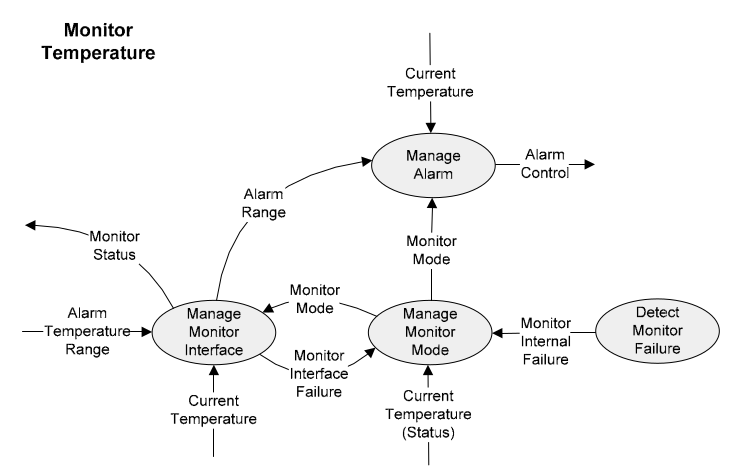
\includegraphics[width=\textwidth]{figures/monitor-temperature-dependency.png}}
  \vspace{-.4cm}
  \caption{Monitor Temperature Dependency Diagram}
  \vspace{-.4cm}
 \label{fig:monitor-temp-dependency}
\end{figure*}

The Monitor Temperature internal variables are shown in table ~\ref{tab:MTI-variables}.

\begin{table}
\begin{tabular}{|l|l|l|l|l|}
\hline
Name & Type & Range & Units & Physical Interpretation \\\hline
Alarm Range &  &  &  & Safe range of Isolette temperature \\\hline
Lower Alarm Temperature & Integer & [96..101] & °F & Lower value of alarm range \\\hline
Upper Alarm Temperature & Integer & [97..102] & °F & Upper value of alarm range \\\hline
Monitor Interface Failure & Boolean & False, True &  & Indicates an operator interface failure \\\hline
Monitor Internal Failure & Boolean & False, True &  & Indicates an internal failure \\\hline
Monitor Mode & Enumerated & Init &  & Initializing following power-up \\\cline{3-5}
  &  & NORMAL &  & Normal mode of operation \\\cline{3-5}
  &  & FAILED &  & Internal failure detected \\\hline
\end{tabular}
\caption{Monitor Temperature Internal Variables}
\label{tab:MTI-variables}
\end{table}

\subsection{Manage Monitor Interface Function}
\label{subsec:MMIF}

The Manage Monitor Interface function defines the interaction with the Operator Interface
external entity. These include obtaining the Alarm Range and reporting back the status of the
Monitor Temperature Function. The constants are shown in table ~\ref{tab:MMIF-constants}.

\begin{table}
\begin{tabular}{|l|l|l|l|l|}
\hline
Name & Type & Range & Units & Physical Interpretation \\\hline
Max Operator & Real & 0.5 & Sec & This time an operation will tolerate between an operator \\
Response Time &  &  &  & request or a change in the Thermostat state and the \\
  &  &  &  & visible response \\\hline
\multicolumn{5}{|l|}{Rationale: A trade study has shown that this lag should be no more than 0.5 second.} \\\hline
\end{tabular}
\caption{The Manage Monitor Interface Function Constants}
\label{tab:MMIF-constants}
\end{table}

The requirements for the Monitor Status controlled variable are as follows:

\begin{itemize}
\item REQ-MMI-1: If the Manage Monitor Interface mode is INIT, the Monitor Status shall be
      set to Init.
\item REQ-MMI-2: If the Manage Monitor Interface mode is NORMAL, the Monitor Status
      shall be set to On.
\item REQ-MMI-3: If the Manage Monitor Interface mode is FAILED, the Monitor Status
      shall be set to Failed.

      Latency: $<$ Max Operator Response Time

      Tolerance: N/A
\end{itemize}

The requirements for Monitor Interface Failure internal variable are as follows:

\begin{itemize}

\item REQ-MMI-4: If the Status attribute of the Lower Alarm Temperature or the Upper
      Alarm Temperature is Invalid, the Monitor Interface Failure shall be set to True.
\item REQ-MMI-5: If the Status attribute of the Lower Alarm Temperature and the Upper
      Alarm Temperature is Valid, the Monitor Interface Failure shall be set to False.

      Rationale: The Monitor Interface Failure internal variable indicates if any errors have
      occurred in sensing the Operator Interface monitored variables needed by the Manage
      Temperature Function. Note that its initial value on power-up will always be True since
      the Status attribute of the Lower Alarm Temperature and the Upper Alarm Temperature
      will initially be Invalid.
\end{itemize}

The requirements for Alarm Range Internal variable are as follows:

\begin{itemize}
\item REQ-MMI-6: If the Monitor Interface Failure is False, the Alarm Range variable shall
      be set to the Desired Temperature Range.
\item REQ-MMI-7: If the Monitor Interface Failure is True, the Alarm Range variable is
      UNSPECIFIED.

      Rationale: The Alarm Range variable is only meaningful when there is not a Monitor
      Interface Failure. If there is, its value should not used and it can be set to any value.
\end{itemize}

\subsection{Manage Monitor Mode Function}
\label{subsec:MMMF}

The Manage Monitor Mode Function determines the mode of the Monitor Temperature
Function. The constants and definitions are shown in tables ~\ref{tab:MMMF-constants} and ~\ref{tab:MMMF-definitions}, respectively.

\begin{table}
\begin{tabular}{|l|l|l|l|l|}
\hline
Name & Type & Range & Units & Physical Interpretation \\\hline
Monitor & Real & 1.0 & Sec & The time allowed for initialization of the Monitor \\
Initialization &  &  &  & Temperature Function before declaring failure \\
Timeout &  &  &  &  \\\hline
\multicolumn{5}{|l|}{Rationale: A trade study has shown that users become impatient if the Thermostat requires} \\
\multicolumn{5}{|l|}{more than one second to initialize.} \\\hline
\end{tabular}
\caption{The Manage Monitor Mode Function Constants}
\label{tab:MMMF-constants}
\end{table}

\begin{table}
\begin{tabular}{|l|l|l|}
\hline
Name & Type & Definition \\\hline
Monitor Status & Boolean & NOT (Monitor Interface Failure OR Monitor Internal Failure) \\
  &  & AND Current Temperature.Status = Valid \\\hline
\end{tabular}
\caption{The Manage Monitor Mode Function Definitions}
\label{tab:MMMF-definitions}
\end{table}

The requirements for the Regulator Mode internal variable are as follows:

\begin{itemize}
\item The modes and transitions of the Manage Regulator Mode Function are specified in the
      state transition diagram shown in figure ~\ref{fig:MTMT}. Each transition is a separate requirement
      and is assigned a unique identifier (e.g., Req MRM 1). All transitions are assumed to
      occur in negligible time.

      Rationale: (Req MRM 3 and Req MRM 4) Once the regulator has failed, the only way
      for it to re-enter normal operation is for it to be powered off and on. This ensures that the
      operators are made aware of any transient failures that the regulator may be experiencing.
\end{itemize}

\begin{figure*}[ht]
  \centerline{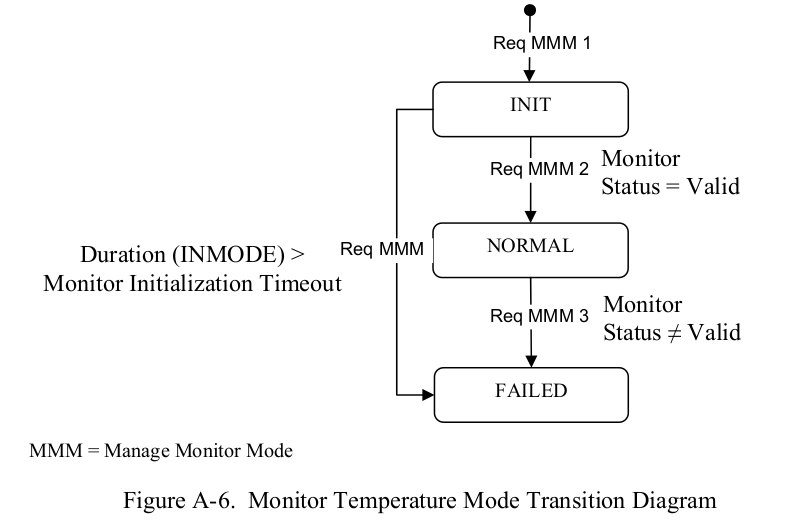
\includegraphics[width=\textwidth]{figures/monitor-temperature-mode-transition.png}}
  \vspace{-.4cm}
  \caption{Monitor Temperature Mode Transition Diagram}
  \vspace{-.4cm}
 \label{fig:MTMT}
\end{figure*}

\subsection{Manage Alarm Function}
\label{subsec:manage-alarm-function}

The Manage Alarm Function turns the Alarm Control on when the Current Temperature of the
Isolette falls below or rises above the Alarm Temperature Range.

The requirements for the Alarm Control controlled variable are as follows:

\begin{itemize}
\item REQ-MA-1: If the Monitor Mode is INIT, the Alarm Control shall be set to Off.

      Rationale: A monitor that is initializing should not activate the alarm unless it enters the
      FAILED mode.
\item REQ-MA-2: If the Monitor Mode is NORMAL and the Current Temperature is less than
      the Lower Alarm Temperature or greater than the Upper Alarm Temperature, the Alarm
      Control shall be set to On.
\item REQ-MA-3: If the Monitor Mode is NORMAL and the Current Temperature is greater
      than or equal to the Lower Alarm Temperature and less than the Lower Alarm
      Temperature +0.5°, or the Current Temperature is greater than the Upper Alarm
      Temperature -0.5° and less than or equal to the Upper Alarm Temperature, the value of
      the Alarm Control shall not be changed.

      Rationale: This provides a hysteresis that prevents transient alarms, see figure ~\ref{fig:alarm-hyperesis}.
\item REQ-MA-4: If the Monitor Mode is NORMAL and the value of the Current
      Temperature is greater than or equal to the Lower Alarm Temperature +0.5° and less than
      or equal to the Upper Alarm Temperature -0.5°, the Alarm Control shall be set to Off.

      Rationale: This turns the alarm off at the same moment that the Displayed Temperature
      shows a value greater than the Lower Alarm Temperature and less than the Upper Alarm
      Temperature.
\item REQ-MA-5: If the Monitor Mode is FAILED, the Alarm Control shall be set to On.

      Rationale: A failed monitor cannot monitor the Current Temperature of the Isolette and
      the Alarm should be turned on.

      Latency: $<$5 seconds

      Tolerance: N/A

      Rationale: Required by SR-2.
\end{itemize}

\begin{figure*}[ht]
  \centerline{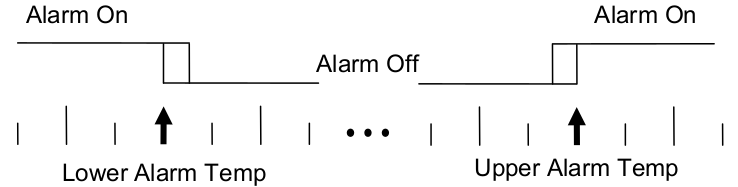
\includegraphics[width=\textwidth]{figures/transient-alarm-hysteresis.png}}
  \vspace{-.4cm}
  \caption{Transient Alarm Hyperesis}
  \vspace{-.4cm}
 \label{fig:alarm-hyperesis}
\end{figure*}

\subsection{Detect Monitor Failure Function}
\label{subsec:DMFF}

The Detect Monitor Failure Function identifies internal failures, (e.g., a memory check failure)
in the Monitor Temperature Function. It defines a single Boolean-valued internal variable,
Monitor Internal Failure, which is set to True if an internal failure is detected.

The requirements for Monitor Internal Failure variable are implementation-specific and cannot
be specified until an implementation platform is chosen.